\chapter{FANET routing protocol}
\label{chap-three}

Each multi-UAV mission has its own set of requirements in terms of size and number of vehicles, the size of the mission's region, payload, mission duration, environmental constraints, level of autonomy and mobility requirements. These all mission-oriented requirements - in turn - generate a peculiar set of demands from the communication infrastructure. Therefore, we will first present an overview of our multi-UAV mission at hand, the communication requirements and then a protocol that facilitates those primitives.

\section{FANET Mission}

The use of multi-cluster UAVs to track gas plumes like volcanic eruptions, forest fires, and environmental contamination has increased in the previous decade. In a plume tracking mission, the UAVs would be required to wrap around the plume, report the contamination level and possibly track the plume by moving along with it. Once the UAVs have been deployed they have complete device autonomy (i.e. each UAV decides its future waypoints and velocity itself using the inputs from onboard sensors and doesn't need these instructions from a human operator) and mission autonomy (i.e. the UAVs must cooperate and coordinate with each other for the successful completion of the mission). It should also be noted that although the UAVs coordinate in the decision-making process, a network-wide consensus might not be required for a specific UAVs operation. As the plume moves in time and space the UAVs should evenly spread out on the surface of the plume while maintaining a safe distance from each other and avoiding any static or dynamic obstacle in their path. 


A detailed description of the problem and a multi-UAV distributed solution has been provided in \cite{8080382}. In the proposed solution the authors have assumed that the mission starts with an initial formation of drones in a 2-dimensional grid (shown in \fref{fig:mesh_formation}). Thereafter, the UAVs move towards the plume autonomously without any ground support. Whenever a UAV detects a contamination it stops and maintains its position with respect to the plume while rest of the UAVs continue their search. If the inter-UAV distance crosses a threshold (too close or too far away) then the moving drone tries to move further or closer to the stationary UAV. These inter-drone forces maintain an approximate mesh structure while resulting in the UAVs wrapping around the plume. As an aid to visualizing this process, think of the mesh as a piece of cloth moving towards a spherical ball and eventually wrapping around the ball. \fref{fig:intermediate_state} shows an intermediate state with drones wrapping around the plume and \fref{fig:final_state} shows a desired final state of UAVs which are wrapped around the plume.
  

\begin{figure}[hbtp]
\centering
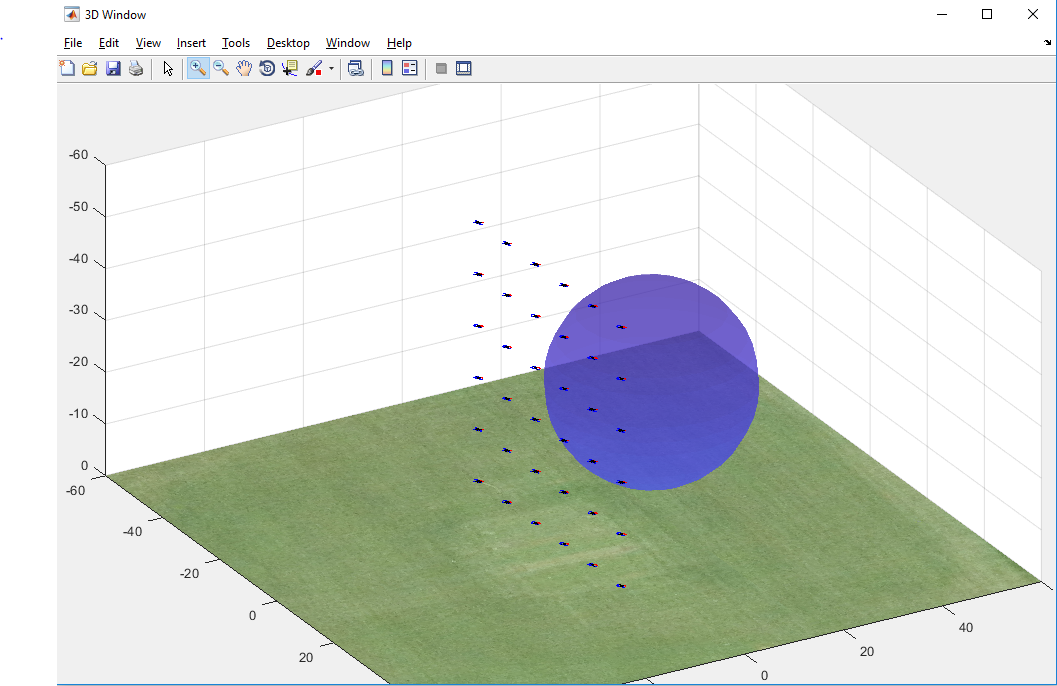
\includegraphics[width=0.8\textwidth]{Chapter-3/figs/initial_drone_config}
\caption{Mesh formation of UAVs at the start of the mission}
\label{fig:mesh_formation}
\end{figure}

\begin{figure}[hbtp]
\centering
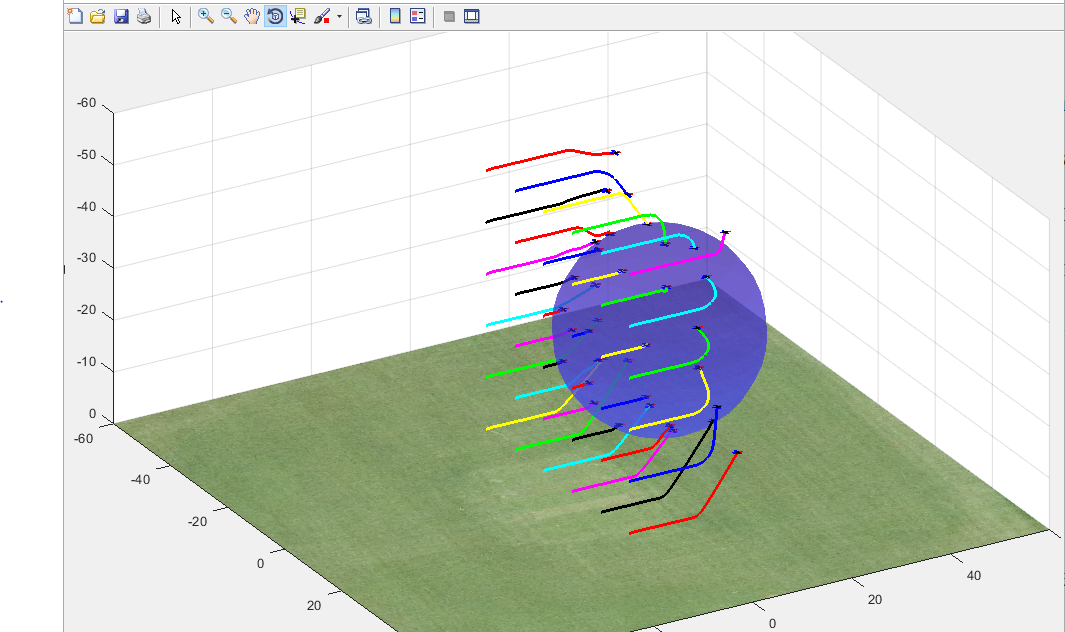
\includegraphics[width=0.8\textwidth]{Chapter-3/figs/intermediate_state}
\caption{UAVs wrapping around the plume. The trailing lines mark the trajectory followed by the UAVs}
\label{fig:intermediate_state}
\end{figure}

\begin{figure}[hbtp]
\centering
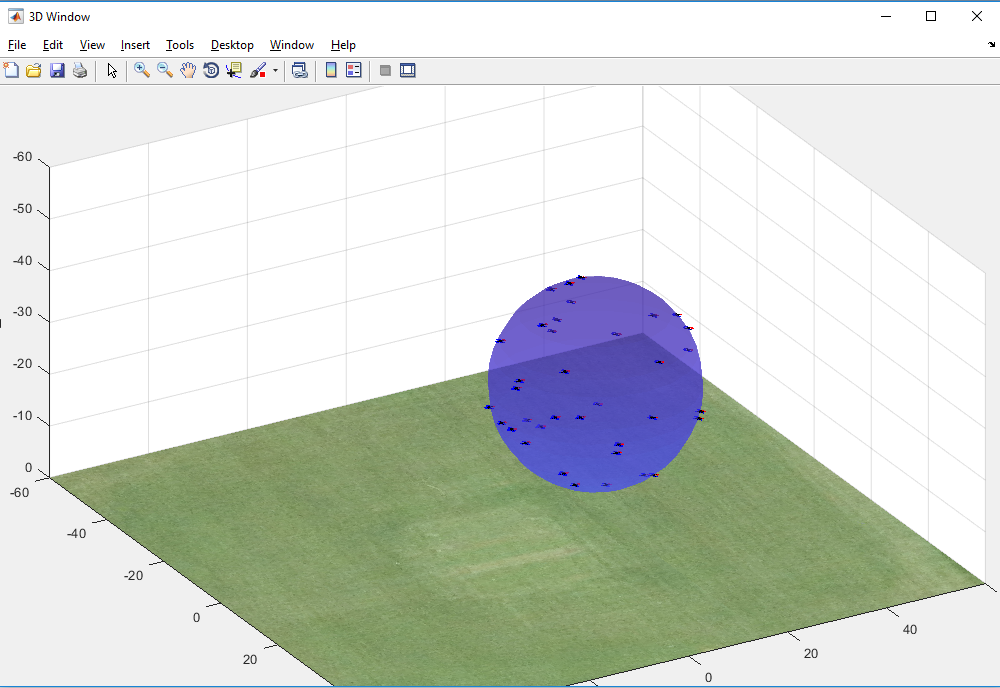
\includegraphics[width=0.8\textwidth]{Chapter-3/figs/final_formation}
\caption{Desired final state of UAVs wrapped around the plume}
\label{fig:final_state}
\end{figure}


\section{Communication requirements} \label{comm_reqs}

In this section, we shall outline the qualitative and quantitative requirements from a communications viewpoint for the successful communication of the mission. We shall use these requirements to design the routing protocol, the message primitives and eventually as a yardstick to measure the performance of the proposed protocol. It should also be noted that the requirements are geared towards a specific mission and since the UAV applications are diverse, these communication demands, and requirements shall widely vary for different applications. For a comprehensive analysis of various civil UAV applications, we refer the readers to \cite{7463007}, where the authors have classified the civil applications of UAVs into four broad categories, namely, Search and Rescue, Area or Network Coverage, Construction, Delivery/transportation and presented the requirements from a communications viewpoint. 

\textbf{Mission coverage:} Applications like plume tracking, wildfire monitoring or plume wrapping typically span a medium to large sized area in the order of tens of kilometers \cite{7463007}. Furthermore, the aerial network should consider the coverage volume expansion or shrinkage with time. The mission volume that we shall be considering would be $ \approx 500 m \times 500 m \times 500 m $. 

\textbf{Network requirement:} Since the mission requires coordination among the participating UAVs, any two participating UAVs should be able to reliably communicate with each other (either directly or multi-hop connectivity). Moreover, the network should be able to reconfigure itself, in other words, the network should consider the nodes joining and leaving the network while the mission is in progress.

\textbf{Number of nodes:} The number of UAVs required in a mission depends on the mission area, transceiver characteristics and the type of nodes employed. Assuming off-the-shelf Wi-fi transceivers and the above mentioned mission coverage the required number of nodes would be around 30. 

\textbf{Connectivity to a base station:} In a real-life deployment scenario, the UAVs must be connected to a base station for safety and security purposes, although the data-rate requirement of the link can be mission specific. In our case, the UAVs need to send their telemetry information (GPS and IMU data) to the base station, however since the mission is fully autonomous with distributed decision-making capacity the entities don't need to relay the coordination data to the base station. A frequency of 4-5 Hz or less is the standard for telemetry data exchange \cite{7463007}. 

\textbf{Connectivity between the other UAVs:} Since the UAVs are required to maintain an approximate mesh structure they need to approximate the distance with other drones. Therefore, the UAVs need to update each other of their GPS locations in real-time. A suitable frequency of this data exchange could be 4-5 Hz. Also, in real deployment scenarios, the UAV cluster can be composed of drones with varying capabilities (UAVs have different sensors) which demands a need for one-to-one communication. Therefore, the UAVs must have a reliable connectivity to each other in either a single or multi-hop fashion. 

\textbf{Collision avoidance:} Once a UAV detects another UAV (e.g. via RADAR) in its flight path, they both need to navigate around each other to avoid a collision. To check if a future waypoint is void of other UAVs, the source UAV can send an anycast to that specific destination region. If some other UAV happens to be in the region then they should negotiate their way around. It should be noted that the originator UAV doesn't know or care about the identity of the drone, rather the message is addressed to the geographical region. This requires a capability to geocast packets where the destination location is the address. These messages are not delay-tolerant and need to be delivered in real time.

\textbf{Group communication:} Sometime a group of UAVs which are a subset of all the UAVs in the network might need to act in accordance of each other. For example, while tracking the plume the UVAs would organize into smaller groups and then move as a cluster around the plume. This would require a mechanism to reach a consensus regarding the group formation, joining or leaving a group and a leader election by the members of the group. 

\textbf{Data type and data rate demands:} The traffic in the aerial UAV network consists of control data (remote controlled data exchange), telemetry data (GPS and IMU data), coordination data (waypoint, mission plan exchange) and sensed data (sensor data). The actual traffic demands depend on the sensor-on-board the UAVs, the type of traffic exchanged in the network and the frequency of such exchange. As per \cite{NASA_UAV_mission_parameters}, imagery and chemical data would need to be collected which would require chemical analyzer, an infrared sensor, image or possibly a video camera. The sensed traffic is sensor dependent and can be, low-rate, bursty or high-rate. In our case, the UAVs need to exchange coordination data among each other, sensed data with the base station and telemetry data with each other as well as the base station. The data exchange with the base station can be periodic and delay-tolerant but the coordination data among the drones must be real-time. As far as data rate is concerned 1 Mbps for images and 2 Mbps for video streaming is sufficient with a typical delay of not more thatn 50-100 ms \cite{7463007}. 

\textbf{Scalability:} The number of nodes can be increased due to two reasons. (1) Increase the coverage volume (2) Increase the density of nodes to get a high-resolution sensory data. A scalabilable network  should handle the increase in a number of nodes/devices in the network and the performance should not degrade unreasonably. 

\textbf{Localization and time synchronization:} The UAVs need to know and report their own location with an accuracy of $\approx 5 m$. This level of accuracy is achievable with off-the-shelf GPS devices and can be improved to a few centimeters by using dual-frequency receivers and/or augmentation systems \cite{gps_accuracy} . The UAVs can also synchronize their clocks through the information provided by GPS.

The above information is summarized in Table \ref{tab:communication_requirements}.
\begin{table}
\caption{Communication requirements}
\label{tab:communication_requirements}
\begin{tabular}{|p{0.38\linewidth}|p{0.47\linewidth}|}
\toprule
Requirements & Values\\
\midrule
Mission Coverage & Medium $\approx 500 m \times 500 m \times 500 m$ or Large\\
\midrule
Network mode & ad hoc \\
\midrule
Number of nodes &  $\approx 30 $ \\
\midrule
Coordination data exchange frequency &  4-5 Hz \cite{7463007}\\
\midrule
Sensed data exchange frequency & 30 Hz for video, 1 Hz for IR and chemical analyzer \cite{7463007}\\
\midrule
Telemetry data exchange frequency & 4-5 Hz \cite{7463007}\\
\midrule
Coordination data link rate (up/down) & 4.8 /64 kbaud \cite{7463007} \\
\midrule
Sensed data link rate (up/down) & 4.8-9.6/64 kbaud for chemical data \cite{NASA_UAV_mission_parameters} 1-2 Mbps for visual data.\\
\midrule
Delay & 50-100 ms \cite{7463007}\\
\midrule
Traffic type & periodic and real time (coordination data, telemetry data), delay tolerant (sensed data) \\
\bottomrule
\end{tabular}
\end{table}

\section{Routing protocol} 
\label{routing_protocol}

\subsection{Protocol description} 
\label{protocol_description}

As we discussed in Chapter \ref{chap-two}, proactively or reactively maintaining routes in tables is not a suitable solution for routing between highly mobile FANET nodes. Therefore a routing scheme which does not maintain end-to-end paths and doesn't employ next-hop forwarding would be more robust. On the other hand, a routing scheme that always floods a packet (nodes discard duplicate receptions to avoid routing loops) in the network doesn't need to maintain any information and is highly robust (i.e. flooding guarantees delivery if the destination node is reachable). However, the associated overhead makes it unsuitable for large and frequent data transfers. 

 A key observation that reduces the number of re-transmissions in flooding is that every node in the network doesn't need to forward a packet for successful delivery; provided some nodes which lie in the direction of the destination node have received and transmitted the packet. For example let's consider a 2 dimensional representation in \fref{fig:routing_motivation}, with source node `S' and destination node `D' the nodes with \emph{black} dots don't need to transmit if the nodes with \emph{red or green} dots have received and transmitted the packet. It should be noted that the red and green dots are closer to the straight line connecting the source and destination node as compared to the black nodes. In this regard we signify the volume enclosing these \emph{`more relevant'} nodes as the \textbf{`transmission zone'}. Therefore, if a source node `S' knows the location of a destination node `D' then `S' can define a transmission zone and restrict re-transmissions to the nodes which lie in the zone, thereby reducing the overhead. This idea of constrained flooding is derived from the concept of the petal in \cite{6133499} and that of request zone in \cite{Ko:1998:LRM:288235.288252}. 

\begin{figure}[hbtp]
\centering
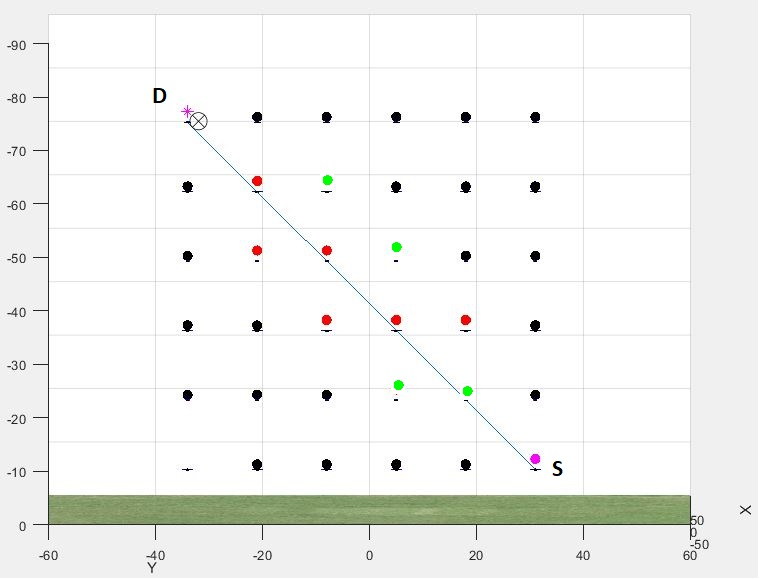
\includegraphics[width=0.5\textwidth]{Chapter-3/figs/routing_motivation}
\caption{Routing protocol motivation. Red and green nodes are closer to the SD lines and hence more relevant for a successful packet delivery}
\label{fig:routing_motivation}
\end{figure}
These `transmission zones' can be defined as different shapes, for example a capsule, cuboid or a spheroid \fref{fig:trans_zones_example} and each have their own peculiar properties. In other words our routing scheme is a restricted flooding algorithm that reduces the overhead by restricting the re-transmissions to a volume between the source and destination nodes. 

\begin{figure}[hbtp]
\centering
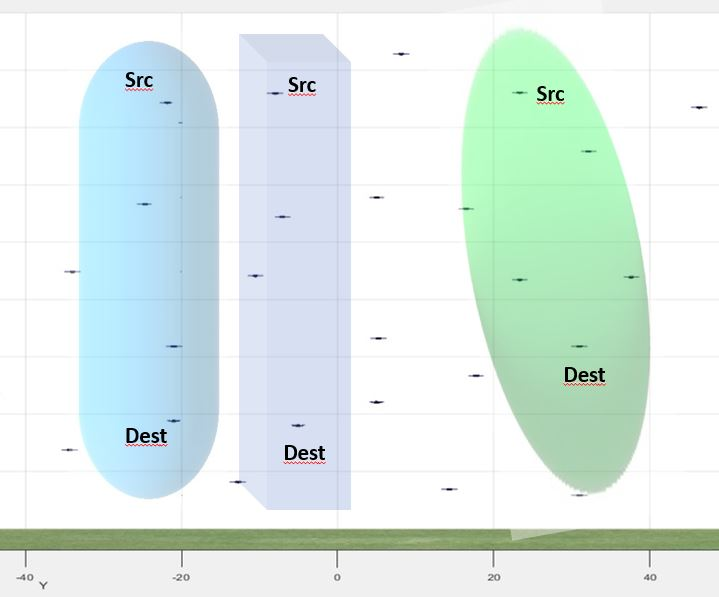
\includegraphics[width=0.5\textwidth]{Chapter-3/figs/Zone_examples}
\caption{Transmission zones to restrict flooding between source and destination}
\label{fig:trans_zones_example}
\end{figure}

We also observe that there is an opportunity to further reduce the number of retransmissions. For example in \fref{fig:routing_motivation} if all the nodes with red dots receive and transmit the packets then even if the nodes with green dots don't re-transmit, the packets shall be successfully delivered to the destination. It should be noted that the red nodes are closer to the source-destination line and also closer to the destination node as compared to the green nodes. This `opportunistic' selection of the nodes can be achieved by introducing a \textbf{`back-off and re-transmit'} mechanism. Specifically, when an intermediate node `N' receives a packet `p', then `N' calculates a `$B_{off}$' time, appends the packet in a waiting queue and registers a callback for the expiry of `$B_{off}$' time. In the meanwhile `N' registers the locations from where `N' heard duplicate transmissions of `p'. After `$B_{off}$' has expired, the node `N' determines the centroid of duplicate transmission locations and if the centroid is closer to the destination compared to the node itself then the node `N' drops the packet otherwise `N' re-transmits the packet. The algorithm to calculate the `back-off' time is presented in Section \ref{back_off_time}. 

\begin{algorithm}
\caption{Schedule received packet: Petal Routing} 
\label{packet_scheduling}
\DontPrintSemicolon
\SetKwProg{Schedule}{Schedule}{}{}

\Schedule{(pkt)}{
    \If{pkt.pId $\in$ transmittedPktIdSet}{
        discard(pkt)\;
        EXIT\;
    }
    
    \If{insideTransmissionZone(pkt, myLoc) == TRUE}{
        \eIf{pkt.pId is in bufWait}{
            Increase duplicate count for pkt.pId\; 
            save pkt.tLoc\;
        }{
            boffTime = calculateBoffTime(pkt)\;
            add pkt to bufWait \;
            
            registerCallback(boffTime, pkt)\;
        }
    }
}
\end{algorithm}

\begin{algorithm}
\caption{Transmit or Drop packet: Petal Routing call-back handler} 
\label{call_back_handler}
\DontPrintSemicolon
\SetKwProg{TransmitOrDrop}{TransmitOrDrop}{}{}
\TransmitOrDrop{(pkt)}{
    dupCoords = duplicateTransmissionCoordinates(pkt)\;
    \eIf {length(dupCoords) > nodeDensity * boundary(dupCoords)}{
        centroid = centroid(dupCoords)\;
        \If{distance(myLoc, pkt.dLoc) < distance(centroid, pkt.dLoc)}{
            discard(pkt)\;
        } {
            pkt.tLoc = myLoc\;
            transmit(pkt)\;
        }
    }{
        pkt.tLoc = myLoc\;
        transmit(pkt)\;
    }
    Add pkt.pId to transmittedPktIdSet\;
}
\end{algorithm}

To this extent, following are the assumptions underlying our routing scheme:

\textbf{Assumptions:}
\begin{enumerate}
\item The wireless antennas on the nodes are omnidirectional.
\item The nodes are reachable from each other i.e. a flooding algorithm can guarantee packet delivery between any pair of nodes and we use the delivery rate of flooding algorithm as an upper bound for our algorithm.
\item The nodes always know their location via GPS. 
\item The nodes synchronize their clock via GPS.
\item A source node knows an approximate location of the destination node which is maintained in a location table and provided by a location service. Different implementations of a location service have been mentioned in Section \ref{loc_service} and our implementation has been explained in Section \ref{loc_service_impl}. 
\item The contention resolution and scheduling issues at the hop time scale are handled by the MAC layer
\end{enumerate}

In a nut-shell, our routing scheme benefits from the inherently broadcast wireless medium and restricts the re-transmissions to a specific volume around the source - destination line and cancelling out redundant transmissions in the process. This routing scheme is presented in Algorithm \ref{packet_scheduling} and \ref{call_back_handler}. A 2D equivalent of our routing scheme is presented in \cite{6133499} and the routing scheme is termed as `petal routing'. Although, all our references are in 3 dimensions, we shall continue the same nomenclature and refer our 3D routing scheme as `Petal routing'.


\subsection{Message primitives} \label{message_primitives}

As discussed in Section \ref{comm_reqs}, the common scenarios when a UAV would need to use the communication service would be the following:

\begin{itemize}
    \item Distribute telemetry data (e.g. GPS, IMU data) with all the UAVs in the network periodically.
    \item Notify all the UAVs in the network of a critical event (e.g. high plume concentration at a location).
    \item Relay telemetry and sensed data to the base station periodically.
    \item Exchange coordination data (e.g. Future waypoint) to UAVs in a specific direction (e.g. to negotiate conflicting paths).
    \item Communication among a group of UAVs for cluster formation, leader election, request to join or exit the cluster. 
    \item Coordinating among the cluster for a consensus on the cluster's behavior.
\end{itemize}

Now we shall present the message primitives that shall facilitate the above communications. 
\begin{enumerate}
\item \emph{NetworkWideFlood(message, sourceID)}: Deliver  the message to all the reachable nodes in the network.
\item \emph{HopLimitedFlood(message, sourceID, HTL)}: Deliver the messages to the neighbouring nodes which are HTL hops away.
\item \emph{Unicast(message, sourceID, destinationID)}: Deliver the message to a specific node.
\item \emph{Geocast(message, sourceID, destinationCoordinates, radius)}: Deliver the message to all the nodes in the specified region.
\item \emph{Multicast(message, sourceID, nodeIDs)}: Deliver the message to all the nodes in the \emph{nodeIDs} list. 
\end{enumerate}

Here \emph{sourceID} and \emph{destinationID} are unique identifiers for a node - possibly IP addresses, while \emph{destinationCoordinates} together with \emph{radius} represent a spherical region with specified coordinate as the center and specified radius. \emph{nodeIDs} is a list containing the ID of nodes in a group. 

We will now present a high-level algorithmic description of these message primitives.

\subsubsection{Network Wide Flood primitive}

Network wide flood primitive ensures that the packet shall be received by all the nodes that are reachable. When a source node `S' needs to send a message to every node in the network, it creates a header with the following parameters and encapsulates the data in this header.

\begin{eqnarray*}
& header = &Header(destId = FLOOD)
\end{eqnarray*} 

Node `S' then broadcasts this message to all its neighbors in the wireless medium. An intermediate node `N', on receiving the message for the first time reads the contents and rebroadcasts it. Thereafter, `N' discards any duplicate receptions of the message. This guarantees that the flooding is loop-free. The benefit of Flooding is the protocol's robustness however there is a high overhead associated with flooding and hence it is suitable for small packets only.

\subsubsection{Hop Limited Flood}

The primitive allows to restrict the span of flooding by the `Hops to Live(HTL)' parameter. For example, if a source node `S' wants to send a message to all its immediate neighbors (i.e. in direct radio range) then `S' shall set the HTL value to 1 in the header. Conceptually, HTL is equivalent to `Time To Live (TTL)' in an IP network. 

\begin{eqnarray*}
& header = &Header(destId = FLOOD, HTL)
\end{eqnarray*} 

It should be noted that hop limited flooding can be used for a network wide flooding by setting HTL equal to infinity (e.g. 15 is assumed to be infinity in RIP). We represent infinity by the macro NETWORK\textunderscore DIAMETER.

The part of receive algorithm that deals with FLOOD packets is depicted in Algorithm \ref{flood_recv}

\begin{algorithm}
\caption{Receive(msg): Flood} 
\label{flood_recv}
\DontPrintSemicolon
\SetKwProg{Receive}{Receive}{}{}
\Receive{(msg)}{%
    \If{msg.pId $\in$ transmittedMsgIdSet}{
        discard(msg)\;
        EXIT\;
    }
    \eIf {msg.destId == FLOOD}{
        \eIf{msg.pId $\notin$ seenIdSet} {
            msg.HTL = msg.HTL - 1\;
            Add (seenIdSet, msg.pId)\;
            \If {msg.HTL > 0}{
                transmit(msg)\;
            }
        }{
            discard(msg)\;
        }
    }{
    ...
    }
}

\end{algorithm}

\subsubsection{Geocast Primitive}

Geocast is used when a UAV wants to communicate with any node present in a geographic region. This is useful in scenarios where two nodes detect a conflicting path and need to negotiate their way around each other.  

When a source node `S' needs to send a message to \emph{any} node in a spherical region `R' with center at \emph{`dLoc'} and radius \emph{`r'} then `S' creates a header with the following parameters.

\begin{eqnarray*}
& header = & Header(destId=ANY, dLoc=[x,y,z], radius=r)
\end{eqnarray*}
Source node `S' then encapsulates the data in this header and transmits the packet. An intermediate node `N' processes the message according to the Algorithm presented in \ref{geocast_recv}

\begin{algorithm}
\caption{Receive(msg): Geocast} 
\label{geocast_recv}
\DontPrintSemicolon
\SetKwProg{Receive}{Receive}{}{}
\Receive{(msg)}{
    \If{msg.pId $\in$ transmittedMsgIdSet}{
        discard(msg)\;
        EXIT\;
    }
    \If{msg.destId == ANY}{
        \eIf{insideDestinationRegion(msg, myLoc)}{
            Transmit(msg)\;
            Add msg.pId to transmittedPktIdSet\;
            EXIT\;
        }{
            Algorithm \ref{packet_scheduling}
        }
    }
}
\end{algorithm}



\subsubsection{Unicast primitive}

Unicast is used when a source node `S' needs to send a message to a destination node `D'. Unicast uses the same underlying mechanism as geocast to route a message except that `S' first consults its location table for `dLoc' - the location of destination `D' - and creates a header with the following parameters.

\begin{eqnarray*}
& header = & Header(destId = destID, dLoc = dLoc)
\end{eqnarray*}
Source node `S' then encapsulates the data in this header and transmits the packet. Moreover, in Unicast the destination is a particular node instead of a regions. An intermediate receiving node `N' follows the Algorithm \ref{unicast_recv}.

\begin{algorithm}
\caption{Receive(msg): Unicast} 
\label{unicast_recv}
\DontPrintSemicolon
\SetKwProg{Receive}{Receive}{}{}
\Receive{(msg)}{
    \If{msg.pId $\in$ transmittedMsgIdSet}{
        discard(msg)\;
        EXIT\;
    }
    \eIf{msg.destId = myId}{
        \If{msg.ackReq == TRUE}{
            ackRep = prepareAckReply()\;
            send(ackRep);
        } 
    }
    {
        algorithm \ref{packet_scheduling}
    }
}
\end{algorithm}


\subsubsection{Multicast primitive}

In our routing scheme,  \emph{multicast} employs \emph{unicast} at application layer i.e. converting a multicast into multiple unicasts --- each one directed to a specific node in the group. Thereby, the receiving end of the algorithm is the same as Algorithm \ref{unicast_recv} whereas the sending part is as depicted in Algorithm \ref{multicast_send} 

\begin{algorithm}
\caption{Send(msg, nodeIDs): Multicast} 
\label{multicast_send}
\DontPrintSemicolon
\SetKwProg{Send}{Send}{}{}
\Send{(msg, nodeIDs)}{
    \ForEach {nodeId $\in$ nodeIDs}{%
        unicast(msg, nodeId)\;
        }
}
\end{algorithm}
